\documentclass[12pt]{article}
\usepackage[english]{babel}

\usepackage{natbib}
\usepackage{tabulary}
\usepackage{ragged2e}
\usepackage{url}
\usepackage[utf8x]{inputenc}
\usepackage{amsmath}
\usepackage{graphicx}
\usepackage{lscape}
\graphicspath{{images/}}
\usepackage{listings}
\usepackage{parskip}
\usepackage{fancyhdr}
\usepackage{vmargin}
\usepackage{pdfpages}
\usepackage{longtable}
\usepackage{wrapfig}
\usepackage{framed}
\usepackage{subcaption}
\usepackage[demo]{graphicx}
\usepackage{amsfonts}

\usepackage{gensymb}
\usepackage{rotating}
\setlength{\parindent}{2em}
\setmarginsrb{3 cm}{2.5 cm}{3 cm}{2.5 cm}{1 cm}{1.5 cm}{1 cm}{1.5 cm}
\setlength{\textwidth}{15.5 cm}
%\setlength{\textheight}{22 cm}

\usepackage{enumitem}
\usepackage{listings}
\usepackage{color}
\usepackage{movie15}
\usepackage{listings}
\usepackage[framed,numbered,autolinebreaks,useliterate]{mcode} % for matlab code
\DeclareMathOperator{\EX}{\mathbb{E}}% expected value
\usepackage[titletoc, title]{appendix}
 
\definecolor{codegreen}{rgb}{0,0.6,0}
\definecolor{codegray}{rgb}{0.5,0.5,0.5}
\definecolor{codepurple}{rgb}{0.58,0,0.82}
\definecolor{backcolour}{rgb}{0.95,0.95,0.92}
 
\lstdefinestyle{mystyle}{
    backgroundcolor=\color{backcolour},   
    commentstyle=\color{codegreen},
    keywordstyle=\color{magenta},
    numberstyle=\tiny\color{codegray},
    stringstyle=\color{codepurple},
    basicstyle=\footnotesize,
    breakatwhitespace=false,         
    breaklines=true,                 
    captionpos=b,                    
    keepspaces=true,                 
    numbers=left,                    
    numbersep=5pt,                  
    showspaces=false,                
    showstringspaces=false,
    showtabs=false,                  
    tabsize=2
}
 
\lstset{style=mystyle}

\usepackage{hyperref}
\hypersetup{
    colorlinks,
    citecolor=black,
    filecolor=black,
    linkcolor=black,
    urlcolor=blue
}


%%%% debut macro %%%%
\makeatletter
\renewcommand{\thefigure}{\ifnum \c@section>\z@ \thesection.\fi
 \@arabic\c@figure}
\@addtoreset{figure}{section}
\makeatother
%%%% fin macro %%%%

%%%% debut macro %%%%
\makeatletter
\renewcommand\theequation{\thesection.\arabic{equation}}
\@addtoreset{equation}{section}
\makeatother
%%%% fin macro %%%%

\title{CHIC Report : Odeji}			% Title
\author{Alexandre Levy & Yves Martin}					% Author
\date{\today}											% Date
% * <antonibigata@yahoo.es> 2017-05-03T09:59:32.665Z:
%
% ^.
\makeatletter
\let\thetitle\@title
\let\theauthor\@author
\let\thedate\@date
\makeatother

\pagestyle{fancy}
\fancyhf{}
% \rhead{}
\lhead{Reconfigurable Robotics Lab \hfill Semester project -- Yves \textsc{Martin}}
\cfoot{\thepage}
\newcommand\norm[1]{\left\lVert#1\right\rVert}
\begin{document}


%%%%%%%%%%%%%%%%%%%%%%%%%%%%%%%%%%%%%%%%%%%%%%%%%%%%%%%%%%%%%%%%%%%%%%%%%%%%%%%%%%%%%%%%%

\begin{titlepage}
	\centering
    % \includegraphics[scale = 0.18]{epfl\_logo2.jpg}\\[0.1 cm]	% University Logo
    % \includegraphics[scale = 0.5]{chic_logo-1.png}\\[0.1 cm]	% University Logo
    % \vspace*{0.8 cm}
	\textsc{\Large Harvard John A. Paulson}\\[0.5 cm]				% Course Code
	\textsc{\Large School of Engineering and Applied Science}\\[0.5 cm]				% Course Name
    \textsc{and}
	\vspace{0.75cm} \\
	\textsc{\Large Ecole Polytechnique Federale de Lausanne}\\[0.5 cm]	
    \rule{5cm}{0.025cm}
    
	\vspace*{0.5 cm}
	
	%\rule{\linewidth}{0.2 mm} \\
	{ \huge \bfseries A Proprioceptive Method for Soft Robots Using Inertial Measurement Units \\[0.1 cm]}
%	\rule{\linewidth}{0.2 mm} \\[1.5 cm]
	
	\centering
	\begin{figure}[ht!]
	    \centering
        
\includegraphics[width=0.3\textwidth]{Docslatex/logo_HMRL.png}
	    \label{fig:my_label}
	\end{figure}


	
		{\large Master's Thesis dissertation  \\ \vspace{0.3cm} April 22$^{nd}$, 2022}\\[2 cm]
		
	\begin{minipage}{0.3\textwidth}
		\begin{flushleft} \large
			\emph{Author:}\\
			Yves \textsc{Martin} \\
			\end{flushleft}
			\end{minipage}~
			\begin{minipage}{0.3\textwidth}
			\centering\large
			\emph{Harvard Supervision:} \\
			Prof. Jaime \textsc{Paik}
			\end{minipage}
			\begin{minipage}{0.3\textwidth}
			\begin{flushright} \large
			\emph{EPFL Supervision:} \\
		    Mustafa \textsc{Mete}\\
		\end{flushright}
	\end{minipage}\\[2 cm]
	
	\leavevmode \\[1cm]
	\vfill

 

	
\end{titlepage}
\renewcommand*\contentsname{Table of contents}
\tableofcontents
\newpage

\section{Abstract}

\begin{itemize}
\item Abstract of the paper
    \item Summary of additional contributions that are not in the paper (shortly)
\end{itemize}


 

\section{Introduction}
% Introductory sentence to summarize the content
\subsection{State of the art}

%% Soft robots are limited by lack of sensors
Proprioception, or the perception of the configuration of one's own body, is essential to robot planning and control.
The configuration of a rigid-bodied robot can be fully described by a finite set of joint displacements which are readily measured using off-the-shelf sensors such as joint encoders.
The configuration of a soft robot, however, is infinite dimensional and cannot readily be measured using off-the-shelf components.

%% Existing soft sensor technologies
To address this shortcoming, a number of sensing technologies have been developed specifically for soft robots \cite{wang2018toward}.
Flexible resistive sensors infer strain by measuring the change in resistance of channels filled with conductive liquids such as liquid metals \cite{park2012design, muth2014embedded} or ionic liquids \cite{helps2018proprioceptive}.
Flexible capacitive sensors estimate changes in geometry by measuring changes in capacitance of stretchable electrodes separated by an elastomeric dielectric layer \cite{yuen2018_strain}.
Optical strain sensors detect changes in geometry by measuring variations in intensity, frequency, or phase of light in a light transmission medium \cite{galloway2019_fiberopt, ZHUANG20187, zhao2016helping, van2018soft}.
Magnetic strain sensors infer displacement by measuring the response of a Hall effect sensor embedded in a soft medium relative to a fixed magnetic field \cite{luo2017_magnet, ozel2015precise}.
Inductive strain sensors estimate changes in geometry by measuring inductance variations caused by transducer mechanisms such as coil geometry and mutual inductance \cite{felt2015contraction, lazarus2018bubble, felt2019inductance}.
Deformable sensing fabrics or ``skins'' that incorporate several soft sensing technologies into a single versatile package have also been developed \cite{case2018_fabrics, Yuen2017_fabric}.

%% FIG: Overview
\begin{figure}
    \centering
    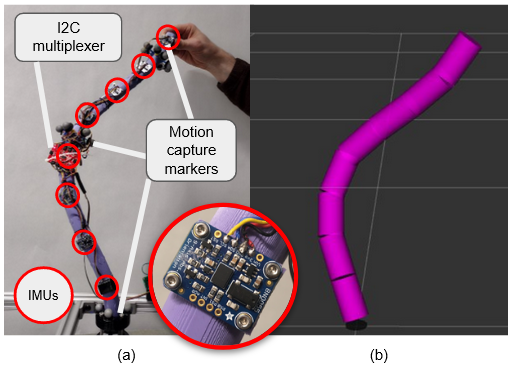
\includegraphics[width=\linewidth]{fig/schematic2.png}
    \caption{(a) The soft arm platform, with IMUs labeled, used to evaluate our estimation methods. (b) A serial-chain rigid-body model approximation of the soft arm motion is shown.}
    \label{fig:schematic}
\end{figure}

%% Current custom soft robot sensors have shortcomings
Each of these sensor types measure the strain of a flexible element.
Using strain measurements to construct an estimate of the pose of a soft arm requires integrating strain along the length, imposing accuracy limitations since small inaccuracies in strain along the length will compound into much larger pose errors.
Furthermore, while each sensor type has its own unique pros and cons, a common issue among them is nonlinear time-variant behavior and hysteresis.
This has motivated the use of machine learning techniques to identify the mapping from raw sensor output to deformation from data \cite{tapia2020_makesense, truby2020_piezo, thuruthel2019soft}.

%% Mocap is an okay alternative but has its own limitations
An alternative to embedded sensors is an external motion capture system.
Such systems utilize an array of externally-mounted infrared cameras to track the position of reflective markers in 3D space.
By coating a soft robot in reflective markers one can use motion capture data to estimate the robot’s shape.
Commercial motion capture systems offer an accurate and reliable method for sensing the deformation of soft robots, but they are expensive and impose severe restrictions on the environment in which a robot can operate.
Motion capture systems are not portable, are sensitive to lighting conditions, and are susceptible to errors due to occlusions, making it impossible to use them outside of a controlled laboratory setting.

%% Proposed solution: IMUs
This paper explores the use of Inertial Measurement Units (IMUs) for sensing the shape of continuum soft robots.
IMUs are off-the-shelf orientation sensors that combine a three-axis accelerometer, three-axis gyroscope, and three-axis magnetometer with an on-board sensor fusion algorithm.
Due to their extensive use in smartphones, tablets, and wearable fitness trackers, IMUs have become widely available and inexpensive, and there are many well-developed computational resources for integrating them into robotic systems \cite{ahmad2013reviews}.

%% Other papers that use IMUs for soft robots
Previous work has explored the use of IMUs for proprioception in soft robots.
In \cite{hughes2020sensing}, two IMUs were used in combination with motor encoders to estimate the pose of a single segment continuum body manipulator assuming constant curvature.
In \cite{yirmibesoglu2016hybrid} two IMUs were embedded into the ends of an elastomeric liquid metal strain sensor to form a hybrid sensor capable of measuring the angle of deflection of a soft bending actuator and the joint position of a rigid robot arm. 
In both of these cases, IMUs were combined with other sensor types (i.e. encoders, strain sensors) to estimate the pose of a one segment soft structure. 

%% Summary of contributions
The contribution of this paper is a simple method for estimating the shape of a full continuum arm using only IMUs.
The approach approximates the infinite-dimensional shape of a continuum arm with a finite-dimensional rigid-body model, and does not require any prior training.
In real-world validation experiments, it is shown to estimate end-effector position to within 10\% of arm length of median error, putting its accuracy on par with that of other soft sensors while avoiding the limitations imposed by external motion capture systems.

%% Outline of the rest of paper
The remainder of this paper is organized as follows.
Section \ref{sec:methods} describes how IMU data is utilized to construct an estimate of the shape of a robot arm.
Section \ref{sec:experiments} describes how the performance of the IMU-based sensing approach was evaluated on a real-world soft arm platform.
Section \ref{sec:results} presents the results of these experiments.
Section \ref{sec:discussion} discusses the results, likely sources of error, and potential improvements.
Section \ref{sec:conclusion} offers concluding remarks and proposes several avenues for future work.

\subsection{Our approach}
\input{Chapters/2 introduction/2 our approach}

\section{Methods}
% Introductory sentence to summarize the content
\subsection{Inertial Measurement Units: calibration and sensor fusion}

\begin{itemize}
    \item Sensor fusion
    \item calibration
    \item give performances with/without calibration
\end{itemize}
\subsection{Piecewise Constant Curvature model}
\begin{itemize}
    \item how to interpolate IMus using quaternions, with plots etc
\end{itemize}
\subsection{Rigid-body model}
\begin{itemize}
    \item method itself with terminology
\end{itemize}
\subsection{PCC-extended Rigid-body model}
\begin{itemize}
    \item method itself with terminology
    \item present it as an extension of the RB model
    \item approximate pcc using polygon-based linear approx 
\end{itemize}

\section{Experimentation}
% Introductory sentence to summarize the content
\subsection{Experimental setup}
\begin{itemize}
    \item hardware
    \subitem bno055 datasheet, performances etc
    \subitem MUX
    \subitem arduino performances
    \subitem block diagram
    \subitem I2C performances
    \item mechanics
    \subitem dimensions, max curvature, shape
    \subitem long shape bc this method works well on long distances
\end{itemize}
\subsection{ROS package}
\begin{itemize}
    \item libraries I used
    \item modules and main function descriptions
    \item performances
    \item how to install it
\end{itemize}
\subsection{Data acquisition}
\begin{itemize}
    \item experimental conditions  
    \item amount of acquired data
\end{itemize}

\section{Results}
% Introductory sentence to summarize the content
\subsection{Main Takeaways}
\input{Chapters/5 results/1 main takeaways}
\subsection{Results of the Rigid-body model}
\input{Chapters/5 results/2 rigid body}
\subsection{Results for the PCC-extended Rigid-body model}
\input{Chapters/5 results/3 pcc ext RB}


\section{Discussion}
% Introductory sentence to summarize the content
\subsection{Performances compared to the existing technologies}
\begin{itemize}
    \item rappel des performances proposees aux results
    \item comparison with previous techniques (in terms of performance)
\end{itemize}
\subsection{Sources of error}
\begin{itemize}
    \item precision de l'IMU
    \item modeling approximatif
    \item comportement non-pcc du bras
\end{itemize}
essayer de quantifier la part de chacun de ces parametres dans l'erreur 
\subsection{Possible applications}
\begin{itemize}
    \item Dan's arm
    \item any long, soft length or surface like wearables
    \item good to capture absolute-oriented shapes
\end{itemize}

\section{Conclusion}
% Introductory sentence to summarize the content



\section{Acknowledgements}
% Introductory sentence to summarize the content\
\begin{itemize}
    \item Dan
    \item Rob
    \item Bouri
    \item Clark and overall the Wood lab
    \item NASA
\end{itemize}

%\newpage
%\section{Annexes}

\section{Bibliography}
\bibliography{bibli} 
\bibliographystyle{ieeetr}
\end{document}

